% Autor: Leonhard Segger, Alexander Neuwirth
% Datum: 2017-10-30
\documentclass[
	% Papierformat
	a4paper,
	% Schriftgröße (beliebige Größen mit „fontsize=Xpt“)
	12pt,
	% Schreibt die Papiergröße korrekt ins Ausgabedokument
	pagesize,
	% Sprache für z.B. Babel
	ngerman
]{scrartcl}

% Achtung: Die Reihenfolge der Pakete kann (leider) wichtig sein!
% Insbesondere sollten (so wie hier) babel, fontenc und inputenc (in dieser
% Reihenfolge) als Erstes und hyperref und cleveref (Reihenfolge auch hier
% beachten) als Letztes geladen werden!

\usepackage{tikz}
\usetikzlibrary{backgrounds,calc,patterns,angles,quotes} % loads some tikz extensions\usepackage{tikz}
\usetikzlibrary{babel}
% Silbentrennung etc.; Sprache wird durch Option bei \documentclass festgelegt
\usepackage{babel}
% Verwendung der Zeichentabelle T1 (Sonderzeichen etc.)
\usepackage[T1]{fontenc}
% Legt die Zeichenkodierung der Eingabedatei fest, z.B. UTF-8
\usepackage[utf8]{inputenc}
% Schriftart
\usepackage{lmodern}
% Zusätzliche Sonderzeichen
\usepackage{textcomp}

% Mathepaket (intlimits: Grenzen über/unter Integralzeichen)
\usepackage[intlimits]{amsmath}
% Ermöglicht die Nutzung von \SI{Zahl}{Einheit} u.a.
\usepackage{siunitx}
% Zum flexiblen Einbinden von Grafiken (\includegraphics)
\usepackage{graphicx}
% Abbildungen im Fließtext
\usepackage{wrapfig}
% Abbildungen nebeneinander (subfigure, subtable)
\usepackage{subcaption}
% Funktionen für Anführungszeichen
\usepackage{csquotes}
\MakeOuterQuote{"}
% Zitieren, Bibliographie
\usepackage{biblatex}


% Zur Darstellung von Webadressen
\usepackage{url}
%chemische Formeln
\usepackage[version=4]{mhchem}
% siunitx: Deutsche Ausgabe, Messfehler getrennt mit ± ausgeben
\usepackage{floatrow}
\floatsetup[table]{capposition=top}
\usepackage{float}
% Verlinkt Textstellen im PDF-Dokument
\usepackage[unicode]{hyperref}
% "Schlaue" Referenzen (nach hyperref laden!)
\usepackage{cleveref}
\sisetup{
	locale=DE,
	separate-uncertainty
}
\bibliography{14Mo_O5_02-07-2018_References}

\begin{document}
	
	\begin{titlepage}
		\centering
		{\scshape\LARGE Versuchsbericht zu \par}
		\vspace{1cm}
		{\scshape\huge O5 - Spektrometer \par}
		\vspace{2.5cm}
		{\LARGE Gruppe 14Mo \par}
		\vspace{0.5cm}
		
		{\large Alexander Neuwirth (E-Mail: a\_neuw01@wwu.de) \par}
		{\large Leonhard Segger (E-Mail: l\_segg03@uni-muenster.de) \par}
		\vfill
		
		durchgeführt am 04.07.2018\par
		betreut von\par
		{\large Johann Preuß} 
		
		\vfill
		
		{\large \today\par}
	\end{titlepage}
	\tableofcontents
	\newpage

	\section{Kurzfassung}
	%TODO Hypothese	und deren Ergebnis, wenn Hypothese ist, dass nur Theorie erfüllt, sagen: Erwartung: Theorie aus einführung (mit reflink) erfüllt
	%TODO Ergebnisse, auch Zahlen, mindestens wenn's halbwegs Sinn ergibt
	%TODO Was wurde gemacht
	%TODO manche leute wollen Passiv oder "man", manche nicht
	
	\section{Methoden}
	%TODO Bilder von der Website klauen
	%TODO einer will Präsens
	
	Zunächst wird das Spektrometer gemäß dessen Anleitung justiert.
	Dabei wird der Prismentisch so ausgerichtet, dass bei Veränderung des Winkels, unter dem das Licht einfällt, die vertikale Position des Spalts im Beobachtungsfernrohr sich nicht verändert.
	Der Spalt wird so schmal gestellt, dass gerade genug Licht durchdringt, als dass er noch gut zu sehen ist.
	Eine Natriumdampflampe wird vor den Spalt gebracht und das Prisma in den Strahlengang gebracht.%TODO irgendwas mit symmetrischer Strahlengang?
	Durch das Fernrohr wird das Linienspektrum beobachtet und jeweils Farbe und ungefähre relative Position notiert.
	
	Dann wird das Prisma durch ein Transmissionsgitter mit $g=\SI{1/300}{mm} $ ersetzt.
	Die Winkelplatte wird so justiert, dass bei Ausrichtung des Fadenkreuzes im Fernrohr auf das Maximum nullter Ordnung ein Winkel von \SI{0}{\degree} gemessen wird.
	Dann werden für eine Drehrichtung für alle erkennbaren Spektrallinien der Winkel abgelesen und, wenn sie erkennbar ist, die Farbe der Linie notiert.
	Dasselbe wird für die erste Ordnung bei einem Gitter mit $g=\SI{1/600}{mm} $ durchgeführt.
	
	Nun wird die Natriumdampflampe durch eine Heliumlampe ersetzt.
	Für diese wird das Winkelspektrum der ersten Ordnung aufgenommen, um später anhand einer Kalibriertabelle die Abhängigkeit von Wellenlänge zu gemessenem Winkel bestimmen zu können. %Winkelspektrum? I guess...
	
	Das Spektrum einer Energiesparlampe wird bei der ersten Ordnung aufgenommen, wobei markiert wird, ob es sich um diskrete Linien oder um ausgeschmierte Bereiche handelt.
	Zuletzt werden die Maxima des Spektrums von verschiedenfarbigen Leuchtdioden aufgenommen und jeweils gemessen, ab welcher Diodenspannung sie sichtbar zu leuchten beginnen. %TODO zu häufg "aufgenommen"?
	
	
	\section{Ergebnisse und Diskussion}
	%TODO Unsicherheiten
	
	
	%TODO Einflüsse von veränderten Parametern auf Messung
	\subsection{Unsicherheiten} %TODO GGF IN DATENANYLSY
	Die Unsicherheiten werden gemäß GUM ermittelt. 
	Außerdem wird für Unsicherheitsrechnungen die Python-Bibliothek "uncertainties" verwendet.
	\begin{description}
		\item[Winkelmessung:] Die Winkel am Spektrometer ließen sich bis auf zwei Nachkommastellen genau analog ablesen. 
		Für das Gitter mit $g=1/\SI{300}{mm}$ und das Prisma, ergibt sich also eine Unsicherheit von \SI{0,002}{\degree} (dreiecke WDF). %weil Analog! 
			Beim Gitter mit $g=1/\SI{600}{mm}$ waren die Maxima nur noch mit einer Unsicherheit von \SI{0,02}{\degree} einem Winkel zuordnen.
	
		\item[Spannungsmessung:] Die Spannung wurde am Multimeter mit zwei Nachkommastellen genau angezeigt, woraus eine Unsicherheit von \SI{0,003}{V} folgt (rechteckige WDF).
			Da die Spannung lediglich zum Messen, wann die LED zu leuchten beginnt und dies mit dem Auge nur grob abgeschätzt werden konnte, verwendet wurde, wurde die Unsicherheit mit \SI{0,03}{V} abgeschätzt.
	\end{description}
	
	\subsection{Natriumdampflampe}
	\subsubsection{Beobachtung und Datenanalyse}
	\subsubsection*{Prisma}
	Die hinter dem Prisma erkennbaren Spektrallinien sind in \cref{fig_draw} skizziert. 
	Die Spektrallinien wurden von links nach rechts stärker gebrochen.
	Auftretende Restlichteffekte ließen sich durch Abschirmung mit beispielweise den Händen entfernen. 
	\begin{figure}[H]
		\centering
		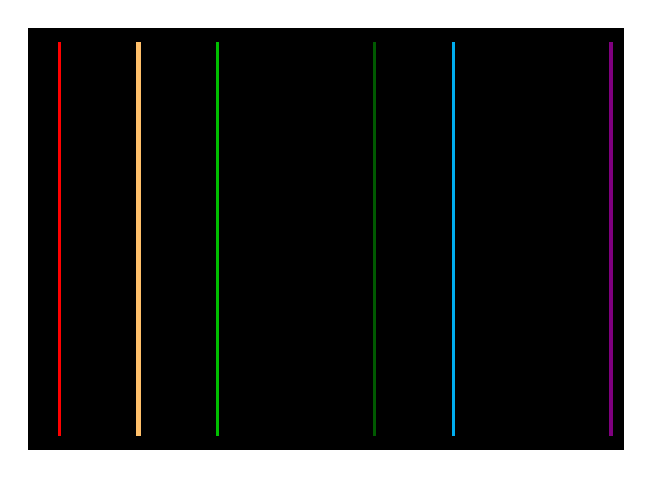
\begin{tikzpicture}[background rectangle/.style={fill=black}, show background rectangle]
			\def\len{5}
			\def\rot{10}
			\def\orange{11}
			\def\gruen{12}
			\def\dgruen{14}
			\def\tuerkis{15}
			\def\lila{17}
			\draw[-,very thick, color=red] (\rot,0) -- (\rot,\len) node [pos=.5,sloped,above] {};
			\draw[-,ultra thick, color={rgb:orange,2;yellow,2;pink,5}] (\orange,0) -- (\orange,\len) node [pos=.5,sloped,above] {};
			\draw[-,very thick, color=black!25!green] (\gruen,0) -- (\gruen,\len) node [pos=.5,sloped,above] {};
			\draw[-,very thick, color=black!65!green] (\dgruen,0) -- (\dgruen,\len) node [pos=.5,sloped,above] {};
			\draw[-,very thick, color=cyan] (\tuerkis,0) -- (\tuerkis,\len) node [pos=.5,sloped,above] {};
			\draw[-,very thick, color=violet] (\lila,0) -- (\lila,\len) node [pos=.5,sloped,above] {};
		\end{tikzpicture}
		\caption{Qualitative Skizze der sichtbaren Spektrallinien der Natriumdampflampe nach Brechung an einem Prisma.} 
		\label{fig_draw}
	\end{figure}
	\subsubsection*{Gitter}
	Die Winkel der Spektrallinien lassen sich mit der Formel aus der Einführung in Wellenlängen umrechnen:
	\begin{equation}
		\lambda = \frac{g \cdot \sin{\vartheta_m}}{m}
		\label{eq_lambda}
	\end{equation}
	\begin{equation}
		u(\lambda) = \left|\frac{g \cdot \cos{\vartheta_m} \cdot u(\vartheta_m)}{m}\right|
	\end{equation}
 	Dabei ist $g$ die Gitterkonstante und $\vartheta_m$ der Beugungswinkel des $m$-ten Beugungsmaximums.
	In \cref{fig_natrium} sind für die Gitter $g=1/\SI{300}{mm}$ und $g=1/\SI{600}{mm}$ die aus den Winkeln resultierenden Wellenlängen verschiedener Ordnungen dargestellt.
	
	\begin{figure}[H] 
		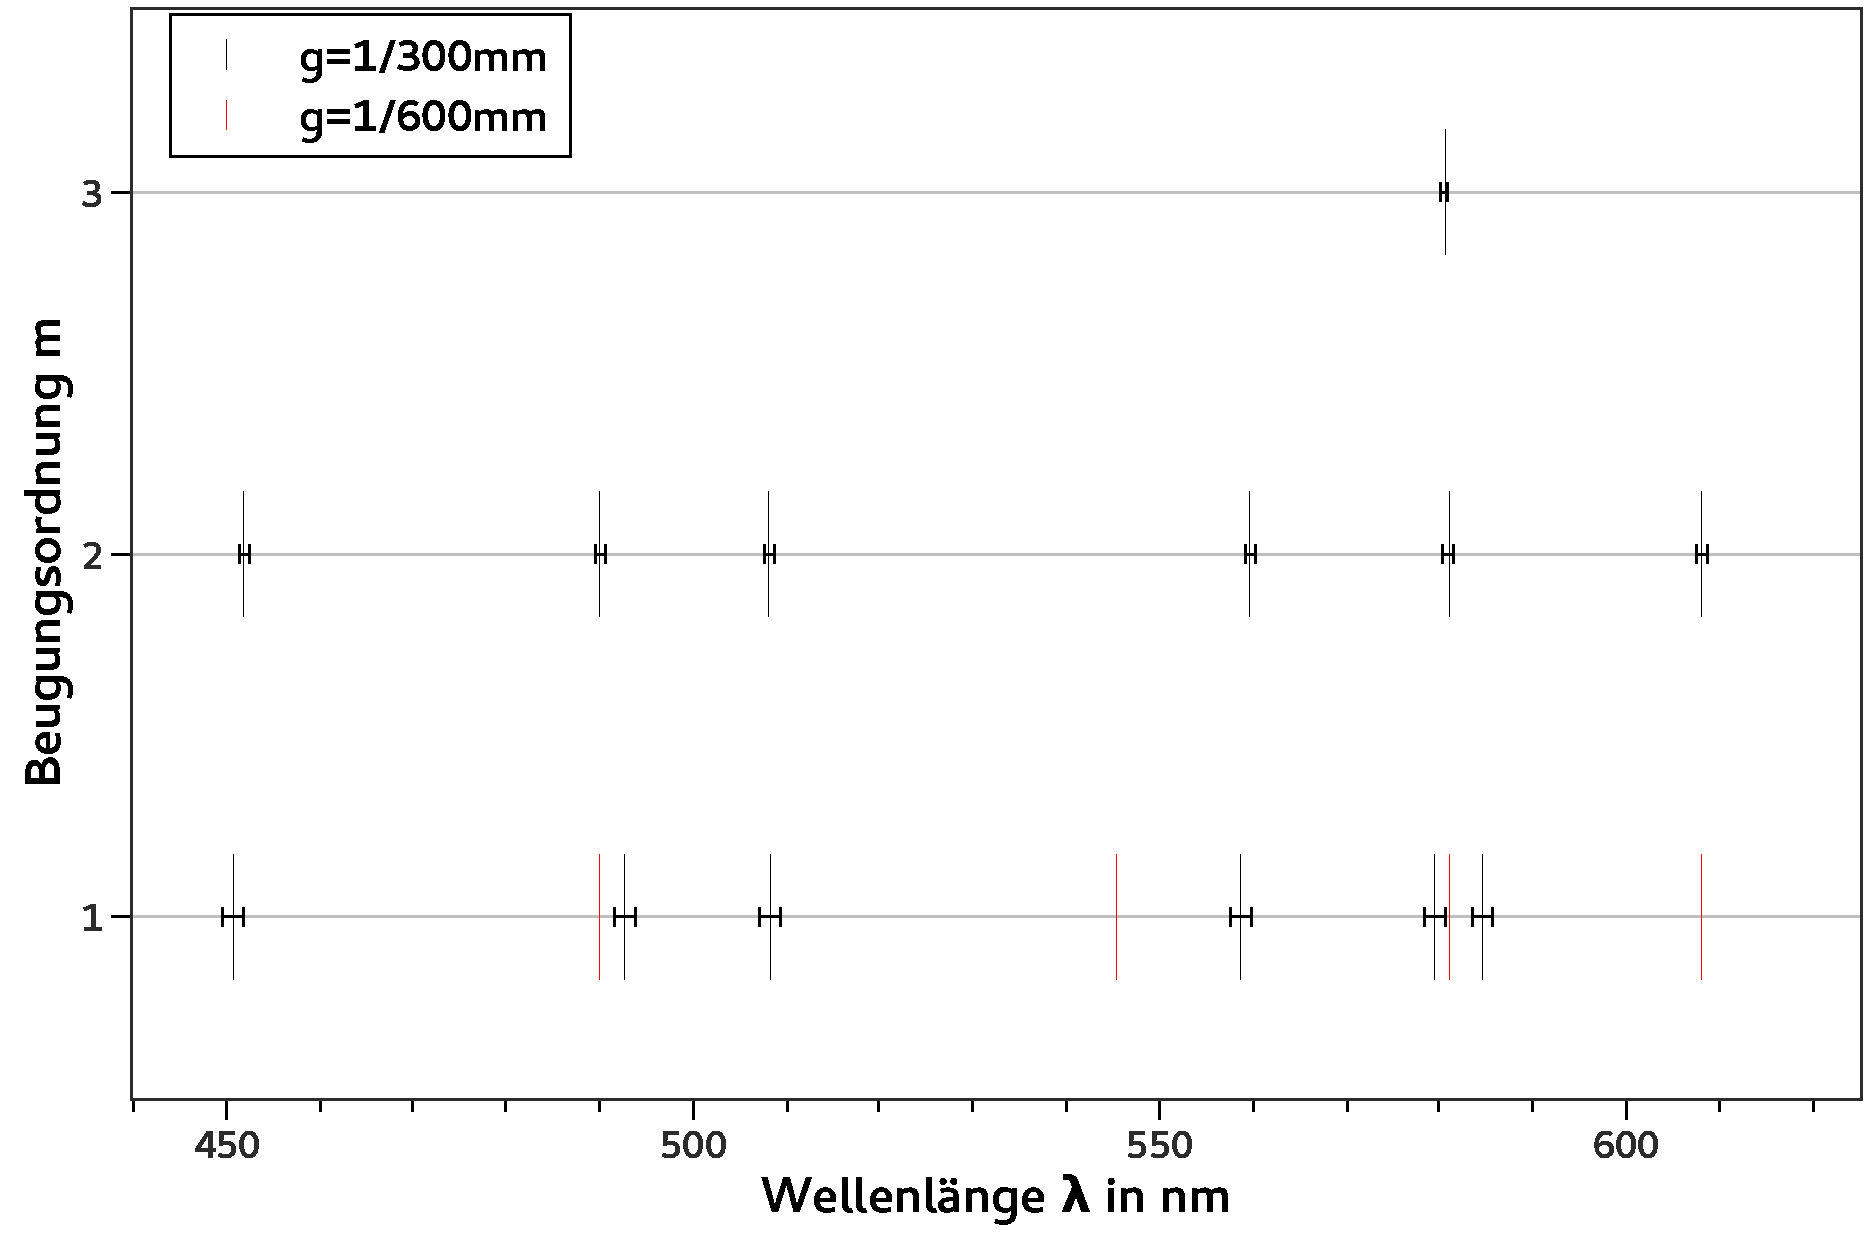
\includegraphics[width=1\textwidth]{fig_natrium}
		\centering
		\caption{Die aus dem Beugungswinkel der Maxima resultierenden Wellenlängen einer Natriumdampflampe sind abgebildet.
		In Schwarz sind die Messwerte beim Gitter mit 300 Spalten pro Millimeter dargestellt und die Rot die vom Gitter mit 600 Spalten pro Millimeter.
		Die Unsicherheit der roten Messpunkte ist kleiner als die Symbolgröße.
		Die Farben entsprechen nicht den beobachteten Farben.
		}
		\label{fig_natrium}
		\centering
	\end{figure}

	\subsubsection{Diskussion}
	
	\cite{NatriumDoppel} gibt an, dass Natrium eine sehr starke Spektrallinie, die Natrium-Doppellinie, bei \SI{589,0}{\nano \meter} und \SI{589,6}{\nano \meter} hat.
	Diese kann durch das Gitter beobachtet werden und auch durch das Prisma lässt sich eine sehr helle Spektrallinie der entsprechenden Färbung erkennen, wie in \cref{fig_natrium} zu erkennen ist.
	Sie kann jedoch in beiden Fällen und auch bei höheren Ordnungen des Gitters nicht in die beiden Teillinien aufgelöst werden.
	Dies ist nicht überraschend, da die Unsicherheit der Wellenlänge bereits größer als die Differenz der Wellenlänge der beiden Linien ist.
	Beim Vergleich der Spektrallinien in den ersten drei Ordnungen fällt zunächst auf, dass in der dritten Beugungsordnung nur noch die Natrium-Doppellinie beobachtet werden kann, was daran liegt, dass die Linien hier nur noch eine so geringe Intensität haben, dass sie mit dem bloßen Auge nicht mehr beobachtet werden können.
	Nur die intensitätsstärkste Linie wird noch gesehen.
	Der Vergleich der beiden Gittern untereinander erlaubt die Feststellung, dass die Linien teilweise beieinander liegen, aber teilweise auch Abweichungen vorhanden sind.
	Die Spektrallinie bei ca. \SI{608}{\nano \meter} konnte beim ersten Gitter nur in zweiter Ordnung gemessen werden, beim zweiten Gitter allerdings auch in erster.
	Dies ist auf sich leicht ändernde Lichtverhältnisse und deshalb nicht immer gleich gute Sichtbarkeit der Spektrallinien durch das Fernrohr zurückzuführen.
	Wenn man das Spektrum insgesamt zwischen Gittern und Prisma vergleicht, stellt man fest, dass die qualitative Darstellung gemäß des Prismas sich auf die Messwerte beim Gitter im Wesentlichen übertragen lässt.
	
	
	\subsection{Heliumlampe} \label{ss_helium}
	\subsubsection{Beobachtung und Datenanalyse}
	In der Einführung ist eine Tabelle zur Kalibrierung des Spektrometers gegeben. %TODO Soll man die angeben, nach Mühlenstrodt scheinbar ja -> Die wollten halt vmtl, dass man die Tabelle mit eingefüllten thetas angibt, not sure, ob wir das tun wollen, wär nicht schlecht i guess, aber nix priority.
	Die Wellenlängen mit einer relativen Intensität von mindestens 100 wurden als die sichtbaren eingestuft, da dies sechs Spektrallinien ergibt und sechs Spektrallinien beobachtet wurden.
	Die Kalibriertabelle beinhaltet zwei rote Spektrallinien, jedoch wurde im Experiment nur eine gemessen.
	Außerdem ließ sich die Spektrallinie geringster Intensität farblich keiner passenden Wellenlänge eindeutig zuordnen, deshalb ergibt sich \cref{fig_helium} aus fünf Messpunkten. %TODO zuordnen? Ist das die, die so dunkel war, dass ich die Farbe nicht erkennen konnte? Wenn ja, ist das merkwürdig formuliert.
	Nach \cref{eq_lambda} würde man eine Sinus-Abhängigkeit erwarten. 
	Ein linearer Fit liegt jedoch deutlich genauer an den Messpunkten, weshalb dieser dienlicher als Kalibrierkurve ist.
	Dies ist erlaubt, weil der Sinus im Rahmen der Kleinwinkelnäherung für kleine Winkel als linear angenommen werden kann.
	Es ist auffällig, dass der Vorfaktor $a$ des Sinus-Fits den erwarteten Wert von 1/\SI{600}{mm} innerhalb seiner Unsicherheiten beinhaltet. 
	Aus $a$ würde durch Umrechnung in 1/\si{mm} eine Gitterkonstante innerhalb des Bereichs von 1/\SI{577}{mm} bis 1/\SI{613}{mm} folgen. %mag ich immer noch nicht.
	

	\begin{figure}[H] 
		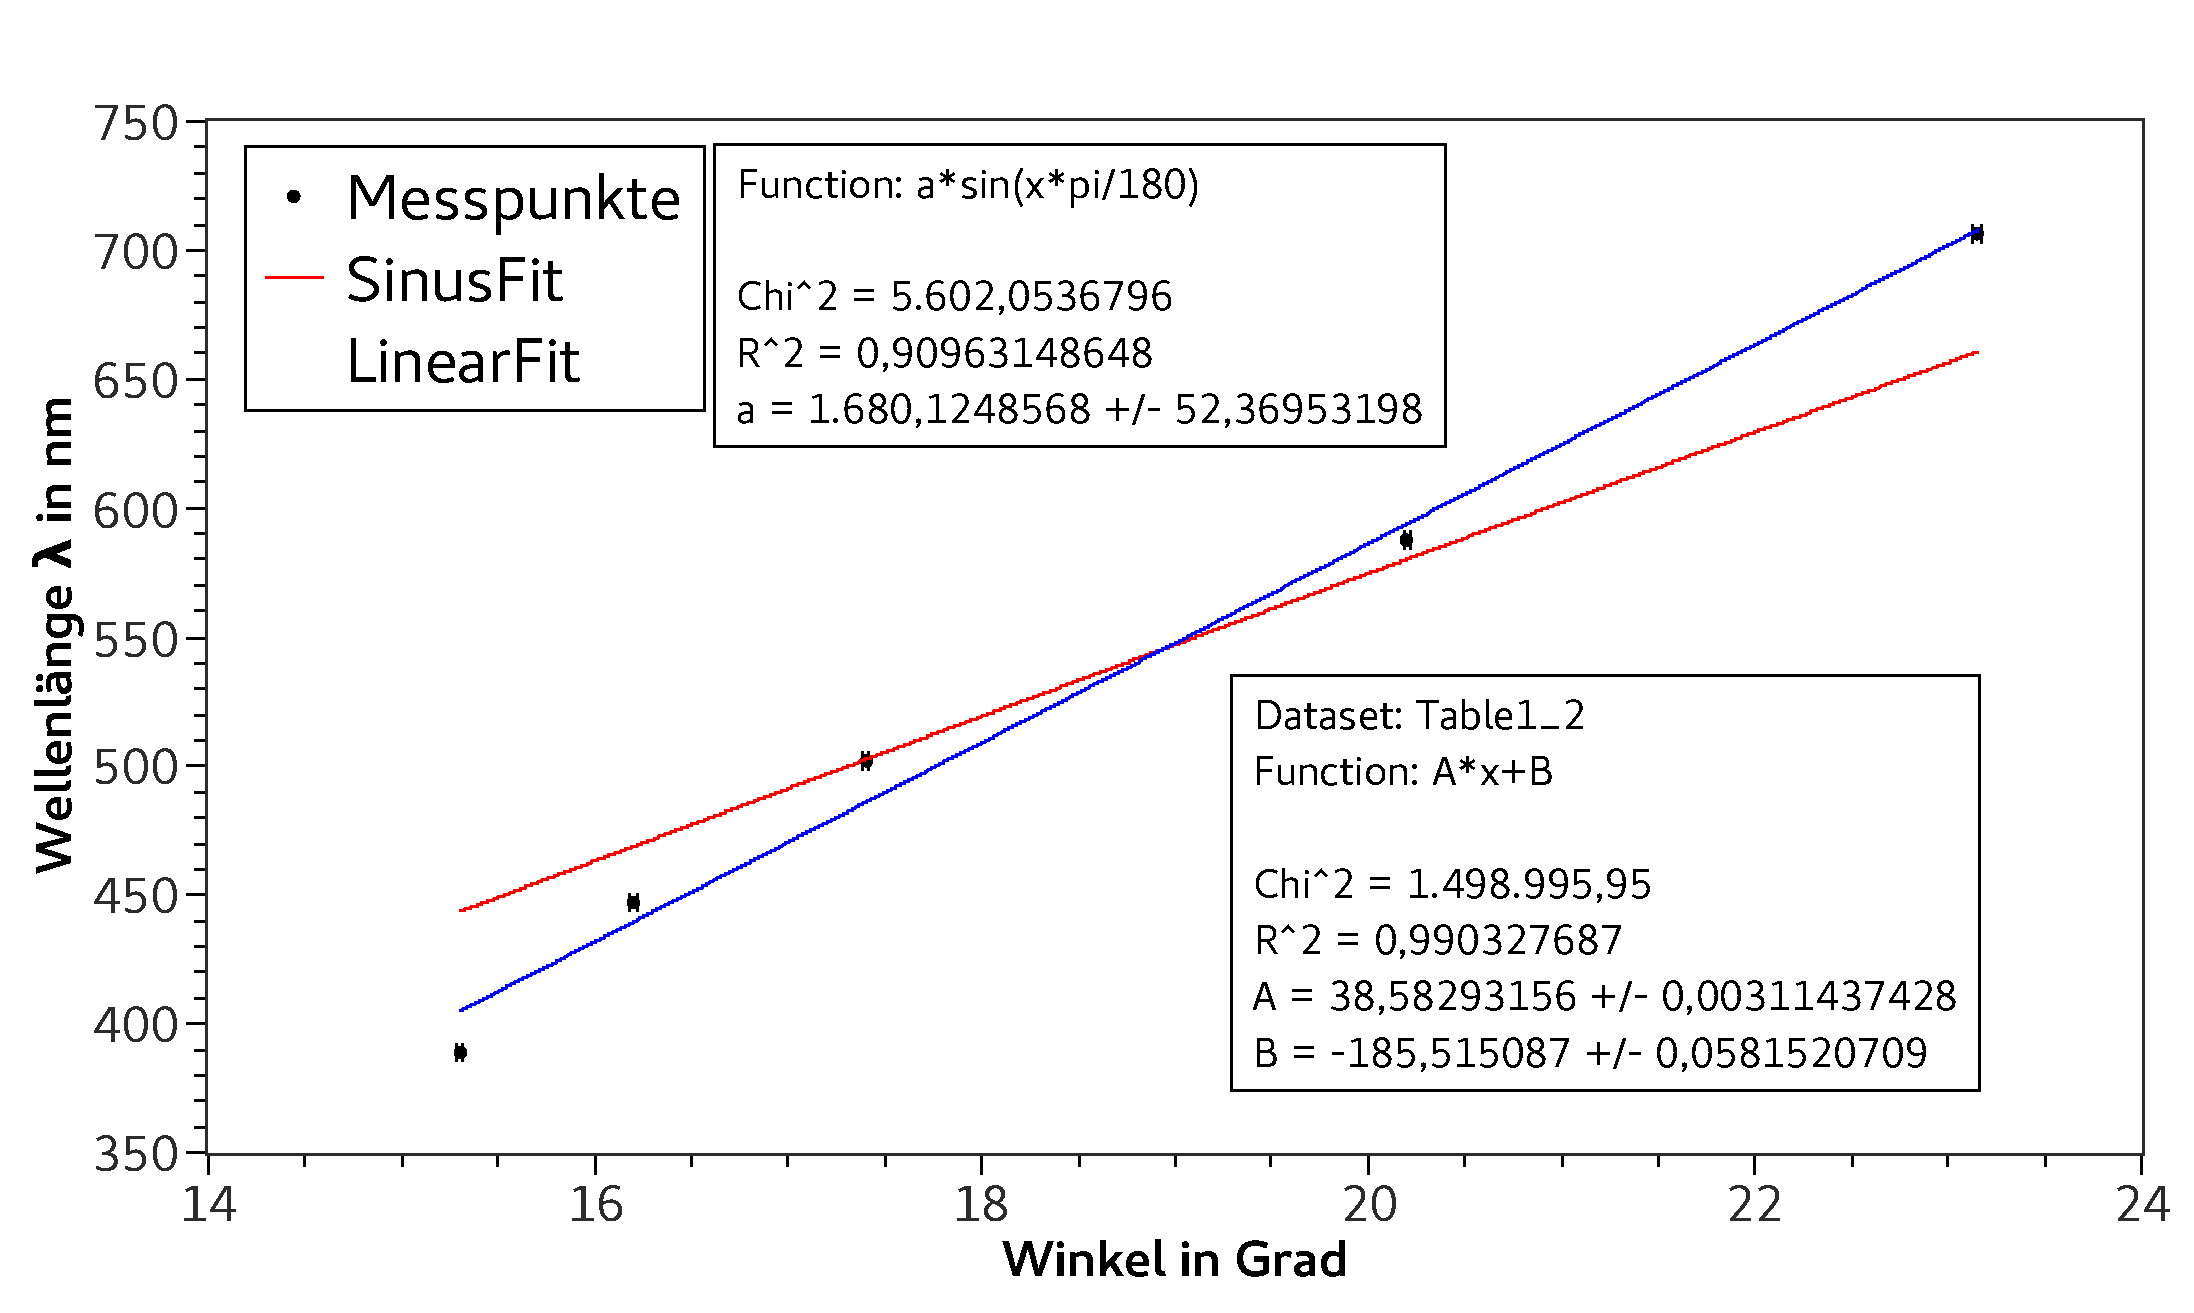
\includegraphics[width=1\textwidth]{fig_helium} 
		\centering
		\caption{Die Wellenlängen der Kalibriertabelle sind gegen die gemessenen Winkel der zugehörigen Spektrallinien aufgetragen.
		Die blaue Funktion ist ein linearer Fit.
		Die rote Funktion ist ein Sinus-Fit.
		Die sich den Fits ergebenden Werte $a$ bzw. $A$ sind dabei in der Einheit Nanometer bzw. Nanometer pro Grad zu verstehen.}
		\label{fig_helium}
		\centering
	\end{figure}

	\subsubsection{Diskussion}
	Die Zuordnung zur Kalibriertabelle wurde dadurch erschwert, dass das menschliche Auge bei geringen Intensitäten keine Farben mehr wahrnimmt, war aber insgesamt möglich.
	Dass einer der Messwerte sich nicht eindeutig einer Kalibrierlinie zuordnen lässt, kann denselben Grund haben.
	%TODO mehr?
	
	\subsection{Energiesparlampe}
	\subsubsection{Beobachtung und Datenanalyse}
	Mithilfe der in \cref{ss_helium} bestimmten Kalibrierkurve lassen sich die Wellenlängen der Spektrallinien der Energiesparlampe ermitteln.
	Diese sind in \cref{fig_spar} dargestellt.


	\begin{figure}[H] 
		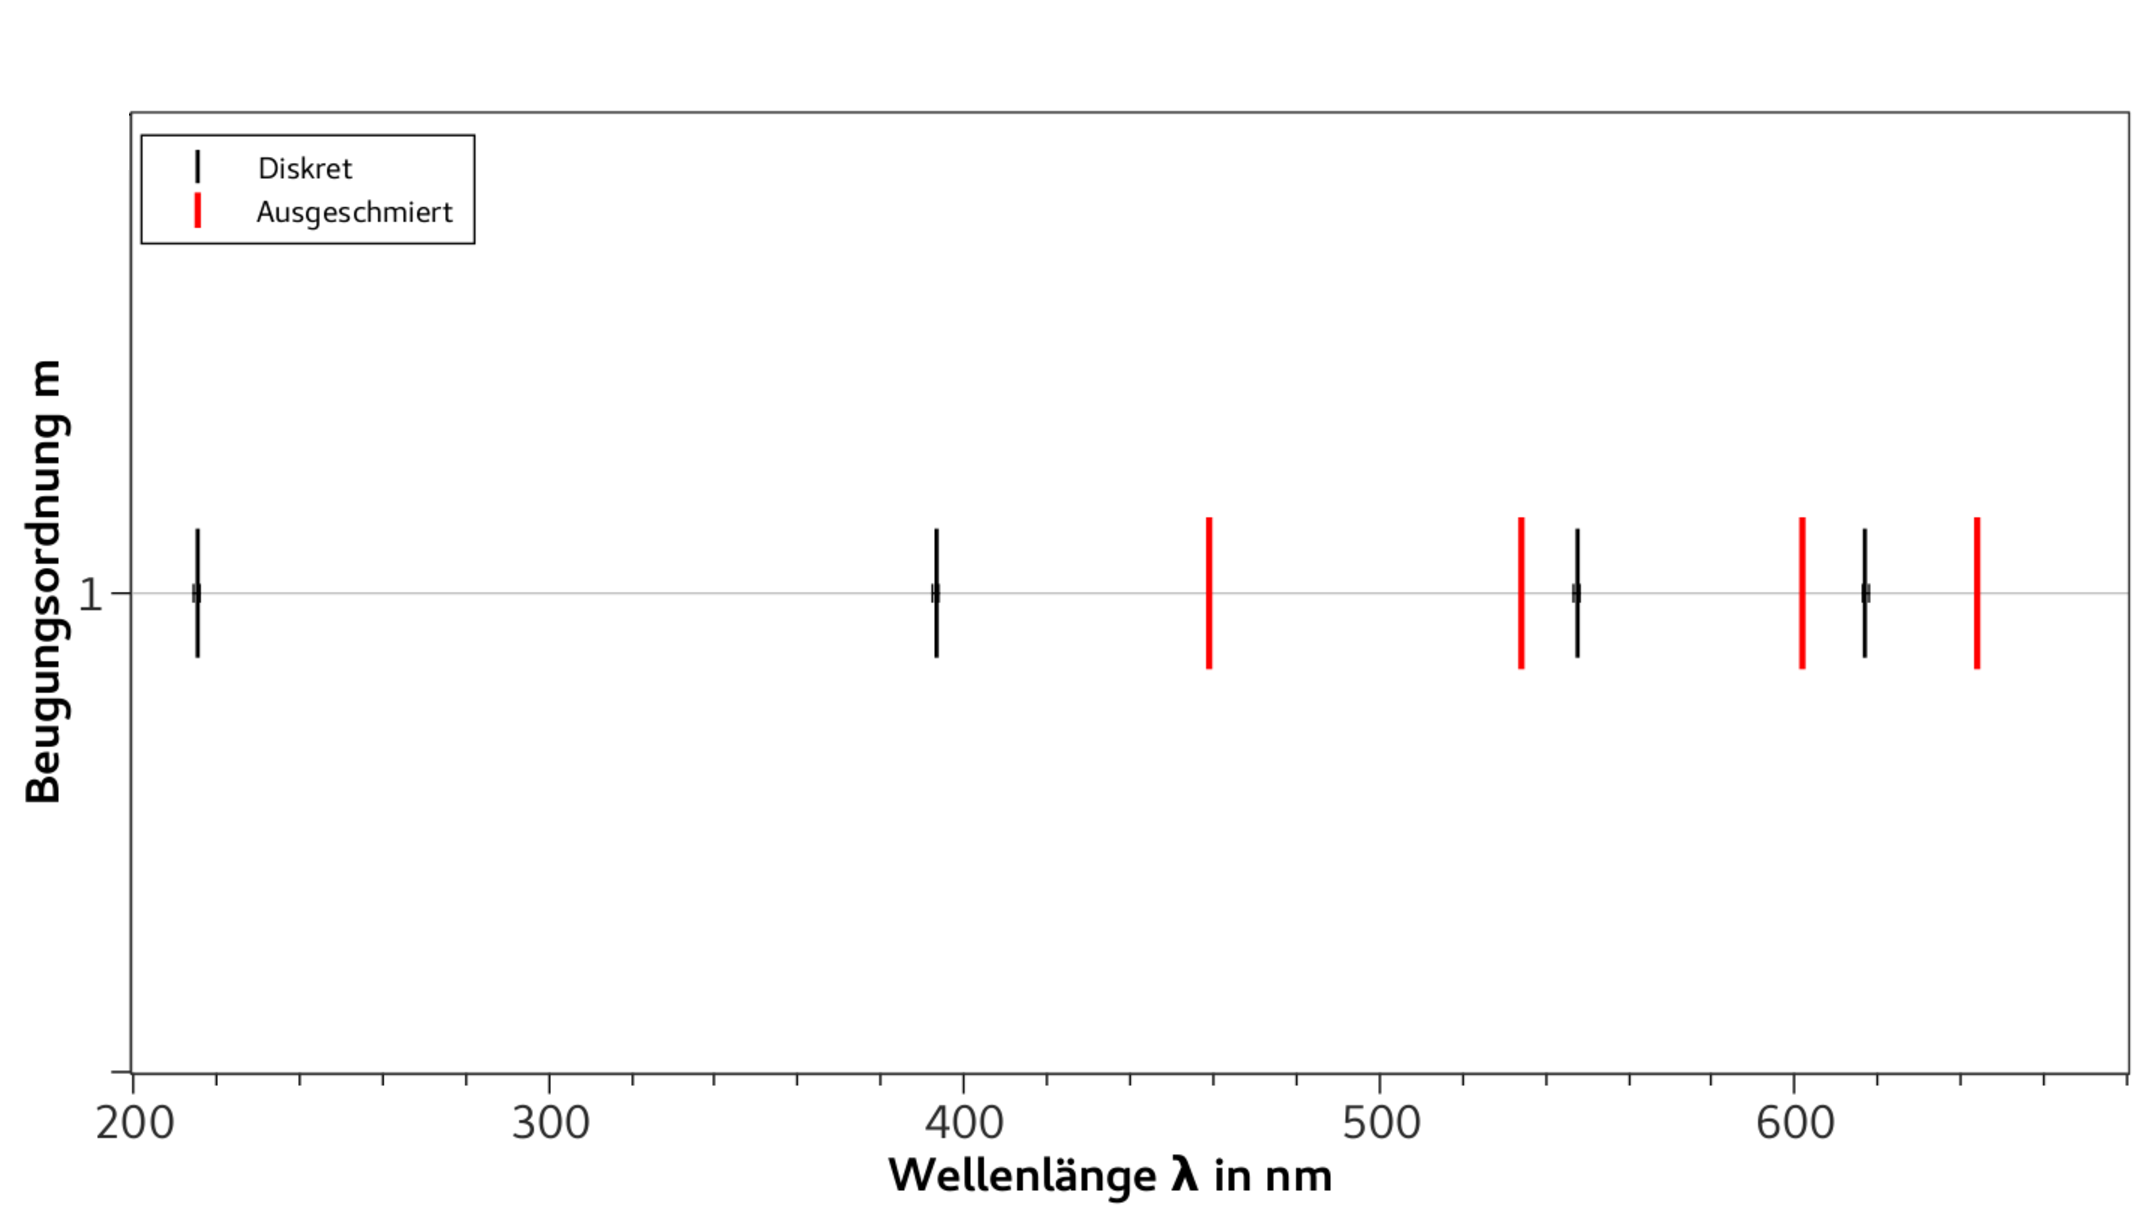
\includegraphics[width=1\textwidth]{fig_spar} 
		\centering
		\caption{Spektrallinien der Energiesparlampe. 
		Es wurden lediglich Maxima der ersten Beugungsordnung beobachtet. %TODO ergo y-Achse unnötig. Außerdem sind das zu viele. Einige sind ja keine Spektrallinien, sondern so ausgeschmierter Bereich. Man soll die die diskreten Spektrallinien bestimmen.
		Die Farben entsprechen nicht den beobachteten Farben.}
		\label{fig_spar}
		\centering
	\end{figure}
	
	\subsubsection{Diskussion}
	%TODO diskrete Spektrallinien -> Gas
	%TODO möglicherweise Mischung aus verschiedenen Leuchtstoffen, Kompaktleuchtstofflampen zählen als Leuchtstofflampen zu den Quecksilberdampf-Niederdrucklampen
	

	\subsection{Leuchtdioden}
	\subsubsection{Beobachtung und Datenanalyse}
	In \cref{fig_led} wurde ein linearer Fit berechnet. 
	Dessen Steigung sollte $hc$ betragen.

	Durch Division von $A$ durch $c$ lässt sich das Plancksche Wirkungsquantum als \SI{5,39 +- 0,92 e-15}{eVs} bestimmen.
	%TODO größere Fehler, weil Maximum nicht eindeutig zu bestimmen und nur grobe Abschätzung!

	\begin{figure}[H] %TODO Groß genug der Fehler? nein->xfehler
		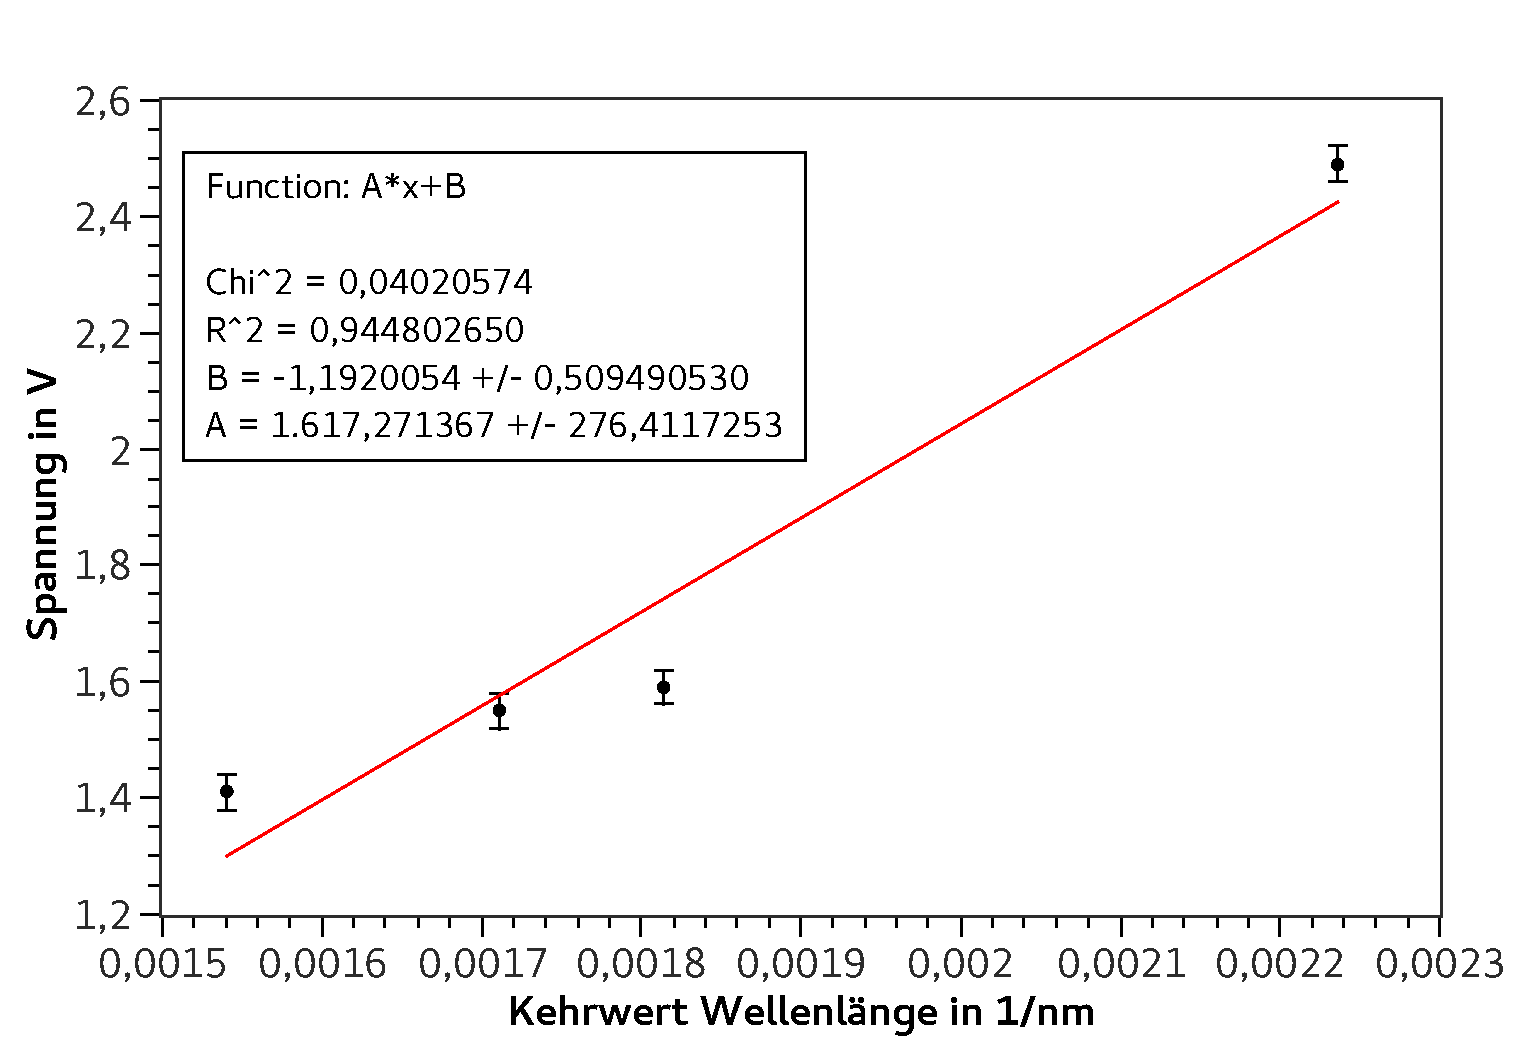
\includegraphics[width=1\textwidth]{fig_led} 
		\centering
		\caption{Die Spannung, ab der die Diode zu leichten beginnt, ist gegen den Kehrwert des Maximums der Emissionswellenlänge aufgetragen.}
		\label{fig_led}
		\centering
	\end{figure}	

	%TODO Berechung nach Aufgabenstellung
	
	\subsubsection{Diskussion}
	
	 %TODO SPLITTEN!
	%TODO Bezug/Nutzen oder sonst was
	%TODO auch hier die Hypothese wiederholen
	%TODO keine Messwerte hier, nach manchen Menschen, zumindest "direkt" erstellte Diagramme net hier, auch wenn Lesbarkeit-bla
	
	%TODO h Literaturvergleich
	
	%TODO Dioden Übergänge so stochastisch, Maximum nicht sehr eindeutig zu bestimmen, keiner sagt, dass Maximum der Bandlücke entspricht, oder? Also eher Minimum der Energie bei Bandlücke?
	
	%TODO alles kann auch einfach Ablesefehler sein, weil ich dumm bin, wenn man noch was braucht
	\section{Schlussfolgerung}
	%TODO Rückgriff auf Hypothese und drittes Nennen dieser
	
	%TODO Quellen zitieren, Websiten mit Zugriffsdatum
	%TODO Verweise auf das Laborbuch (sind erlaubt)
	%TODO Tabelle + Bilder mit Beschriftung
	\printbibliography
\end{document}
